%%%%%%%%%%%%%%%%%%%%%%%%%%%%%%%%%%%%%%%%%%%%%%%%%%%%%%%%%%%%%%%%%%%%%%
% LaTeX Template: Beamer arrows
%
% Source: http://www.texample.net/
% Feel free to distribute this template, but please keep the
% referal to TeXample.net.
% Date: Nov 2006
% 
%%%%%%%%%%%%%%%%%%%%%%%%%%%%%%%%%%%%%%%%%%%%%%%%%%%%%%%%%%%%%%%%%%%%%%
% How to use writeLaTeX: 
%
% You edit the source code here on the left, and the preview on the
% right shows you the result within a few seconds.
%
% Bookmark this page and share the URL with your co-authors. They can
% edit at the same time!
%
% You can upload figures, bibliographies, custom classes and
% styles using the files menu.
%
% If you're new to LaTeX, the wikibook is a great place to start:
% http://en.wikibooks.org/wiki/LaTeX
%
%%%%%%%%%%%%%%%%%%%%%%%%%%%%%%%%%%%%%%%%%%%%%%%%%%%%%%%%%%%%%%%%%%%%%%

\documentclass{beamer}

\usetheme{CambridgeUS}
\usefonttheme{professionalfonts}
\usepackage{times}
\usepackage{tikz}
\usepackage{amsmath}
\usepackage{verbatim}
\usepackage{natbib}
\usepackage[francais]{babel}
\usepackage[T1]{fontenc}
\usepackage[utf8x]{inputenc}
\usepackage{booktabs} % Allows the use of \toprule, \midrule and \bottomrule in tables
\usepackage{graphicx}
\usepackage{wrapfig}
\usepackage{multicol}

\usetikzlibrary{arrows,shapes}

\author{Alexandre Hulsken (CRIStAL / FOX)}
\title{Reconnaissance d'émotions par réseaux de neurones à Spikes}


\begin{comment}
:Title: Beamer arrows
:Tags: Remember picture, Beamer, Physics & chemistry, Overlays
:Use page: 3

With PGF/TikZ version 1.09 and later, it is possible to draw paths between nodes across
different pictures. This is a useful feature for presentations with the
Beamer package. In this example I've combined the new PGF/TikZ's overlay feature
with Beamer overlays. Download the PDF version to see the result.

**Note.** This only works with PDFTeX, and you have to run PDFTeX twice.

| Author: Kjell Magne Fauske

\end{comment}


% For every picture that defines or uses external nodes, you'll have to
% apply the 'remember picture' style. To avoid some typing, we'll apply
% the style to all pictures.
\tikzstyle{every picture}+=[remember picture]

% By default all math in TikZ nodes are set in inline mode. Change this to
% displaystyle so that we don't get small fractions.
\everymath{\displaystyle}

\title[Label Recherche]{Reconnaissance d’émotions par réseaux de neurones à Spikes}

\author{Alexandre Hulsken}
\institute[IRCICA/FOX]
{
Université des Sciences et Technologie de Lille \\
\medskip
%\textit{john@smith.com} % Your email address
}
\date{22 mars 2018}

\begin{document}

\begin{frame}
\titlepage
\vfill
Encadré par :\par
Pierre \textsc{Tirilly} \\
Benjamin \textsc{Allaert}
\end{frame}

%\begin{frame}
%  \frametitle{Sommaire}
%  \tableofcontents
%\end{frame}

%------------------------------------------------
\section{Définir les bases}
%------------------------------------------------

\subsection{Contexte}
\begin{frame}
  \frametitle{Contexte}
  Méthodes tradi reconnaissance emo
  Méthide deep learining => tps
  Nvx modèle SNN
\end{frame}

%------------------------------------------------

\subsection{Problématique}
\begin{frame}
  \frametitle{Problématique}
  \centering
  \huge{Expérimenter les réseaux de neurones à Spikes}
\end{frame}

%------------------------------------------------

\subsection{Définitions}
\begin{frame}
  \frametitle{Définition}
  \begin{block}{Une émotion}
    Il existe différentes manières de représenter une émotion tel que :
    \begin{itemize}
      \item Les émotions d'Ekman
      \item Le FACS
    \end{itemize}
    classif discrète ekman 6 classes (joie peur la surprise la colere degout tristesses) + photos
  \end{block}
\end{frame}

%------------------------------------------------

\subsection{Le principe de reconnaissance d'expressions faciales}
\begin{frame}
  \frametitle{Le principe de la reconnaissance}
  3 étapes:
  \begin{enumerate}
    \item Le prétraitement
    \item L'extraction de modèle
    \item La classification
  \end{enumerate}
  schéma
\end{frame}

%------------------------------------------------
\section{Reconnaître une émotion}
%------------------------------------------------

\subsection{Le prétraitement de la donnée}
fusion avec prec
\begin{frame}
  \frametitle{Le prétraitement}
  \begin{columns}[c] 
    \column{.45\textwidth}
      \textbf{Etapes :}
      \begin{itemize}
        \item Extraction d'une zone
        \item Changement de couleur
        \item Extraction de contours
      \end{itemize}

    \column{.5\textwidth}
      \begin{figure}[position]
      	\centering
        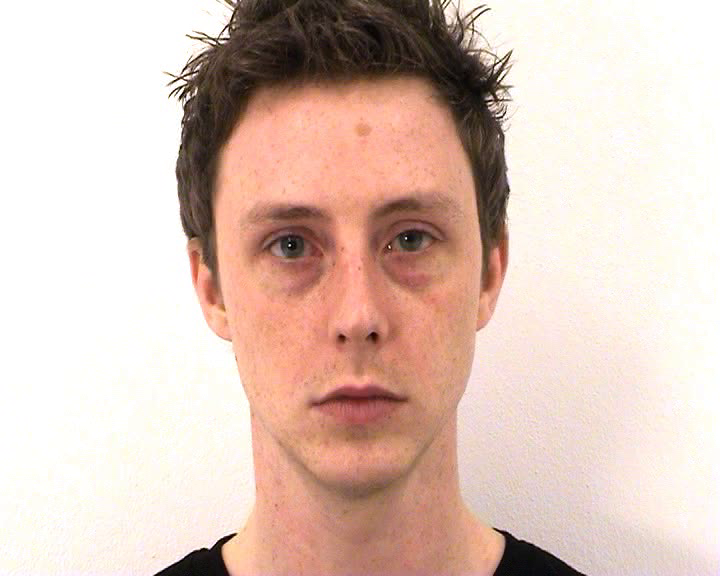
\includegraphics[scale=0.15]{image/img_001.png}
        \vfill
        \vspace{2mm}
        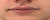
\includegraphics{image/cropped.png}
        \vfill
        \vspace{2mm}
        
\includegraphics{image/grayscale.png}
        \vfill
        \vspace{2mm}
        
\includegraphics{image/dog_on.png}
        \hspace{3mm}
        
\includegraphics{image/dog_off.png}
      \end{figure}
  \end{columns}
\end{frame}

%------------------------------------------------

\subsection{L'extraction de modèles}
\begin{frame}
  \frametitle{Le comportement du neurone}
  \begin{figure}
  	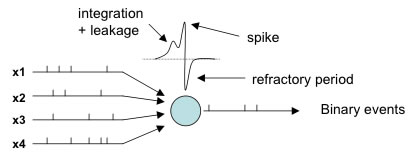
\includegraphics[scale=0.8]{image/neurone.jpg}
  \end{figure}
\end{frame}

%------------------------------------------------

\begin{frame}
  \frametitle{Une architecture de réseau de neurone impulsionnel}
  \begin{figure}
    \centering
    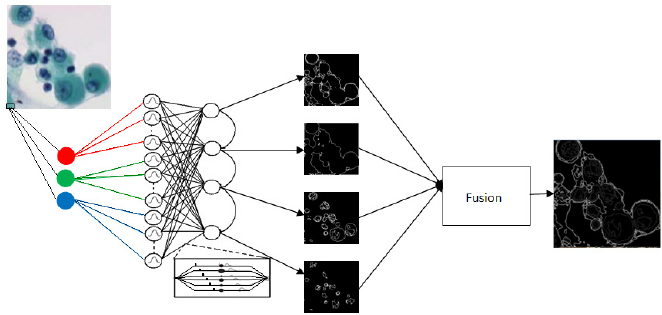
\includegraphics[scale=0.5]{image/SNN1.png}
  \end{figure}
\end{frame}

%------------------------------------------------

\subsection{La classification}
\begin{frame}
	schema SVM
    separatrice lineaire
  \frametitle{La classification}
  \begin{columns}[c]
    \column{.45\textwidth}
      \textbf{3 étapes :}
      \begin{enumerate}
        \item Acquisition
        \item Sélection
        \item Construction
      \end{enumerate}

    \column{.5\textwidth}
      \begin{block}{Définition du classifieur}
      	fonction permettant de reconnaître si un élément se trouve dans un espace
      \end{block}
  \end{columns}
\end{frame}

%------------------------------------------------
\section{Expérimenter l'architecture}
%------------------------------------------------

\subsection{Les choix de critères de réussite}
\begin{frame}
  \frametitle{Les choix de critères de réussite}
  \centering
  plus bas (perspective)
  \Huge{Que choisir?}
\end{frame}
%------------------------------------------------

\subsection{Test de difficulté}
\begin{frame}
  \frametitle{Test de difficulté}
    \begin{columns}
      \column[c]{.5\textwidth}
        \begin{figure}
        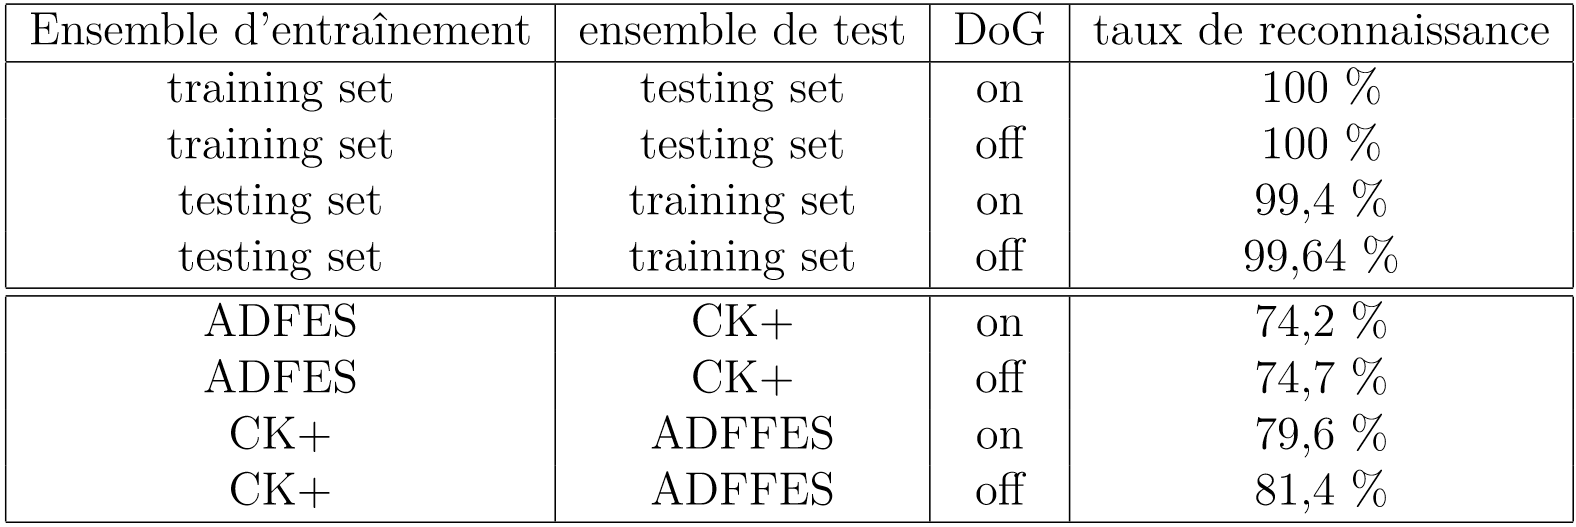
\includegraphics[scale=0.15]{image/resultat_exp.png}
        \end{figure}

      \column[c]{.5\textwidth}
        \begin{figure}
        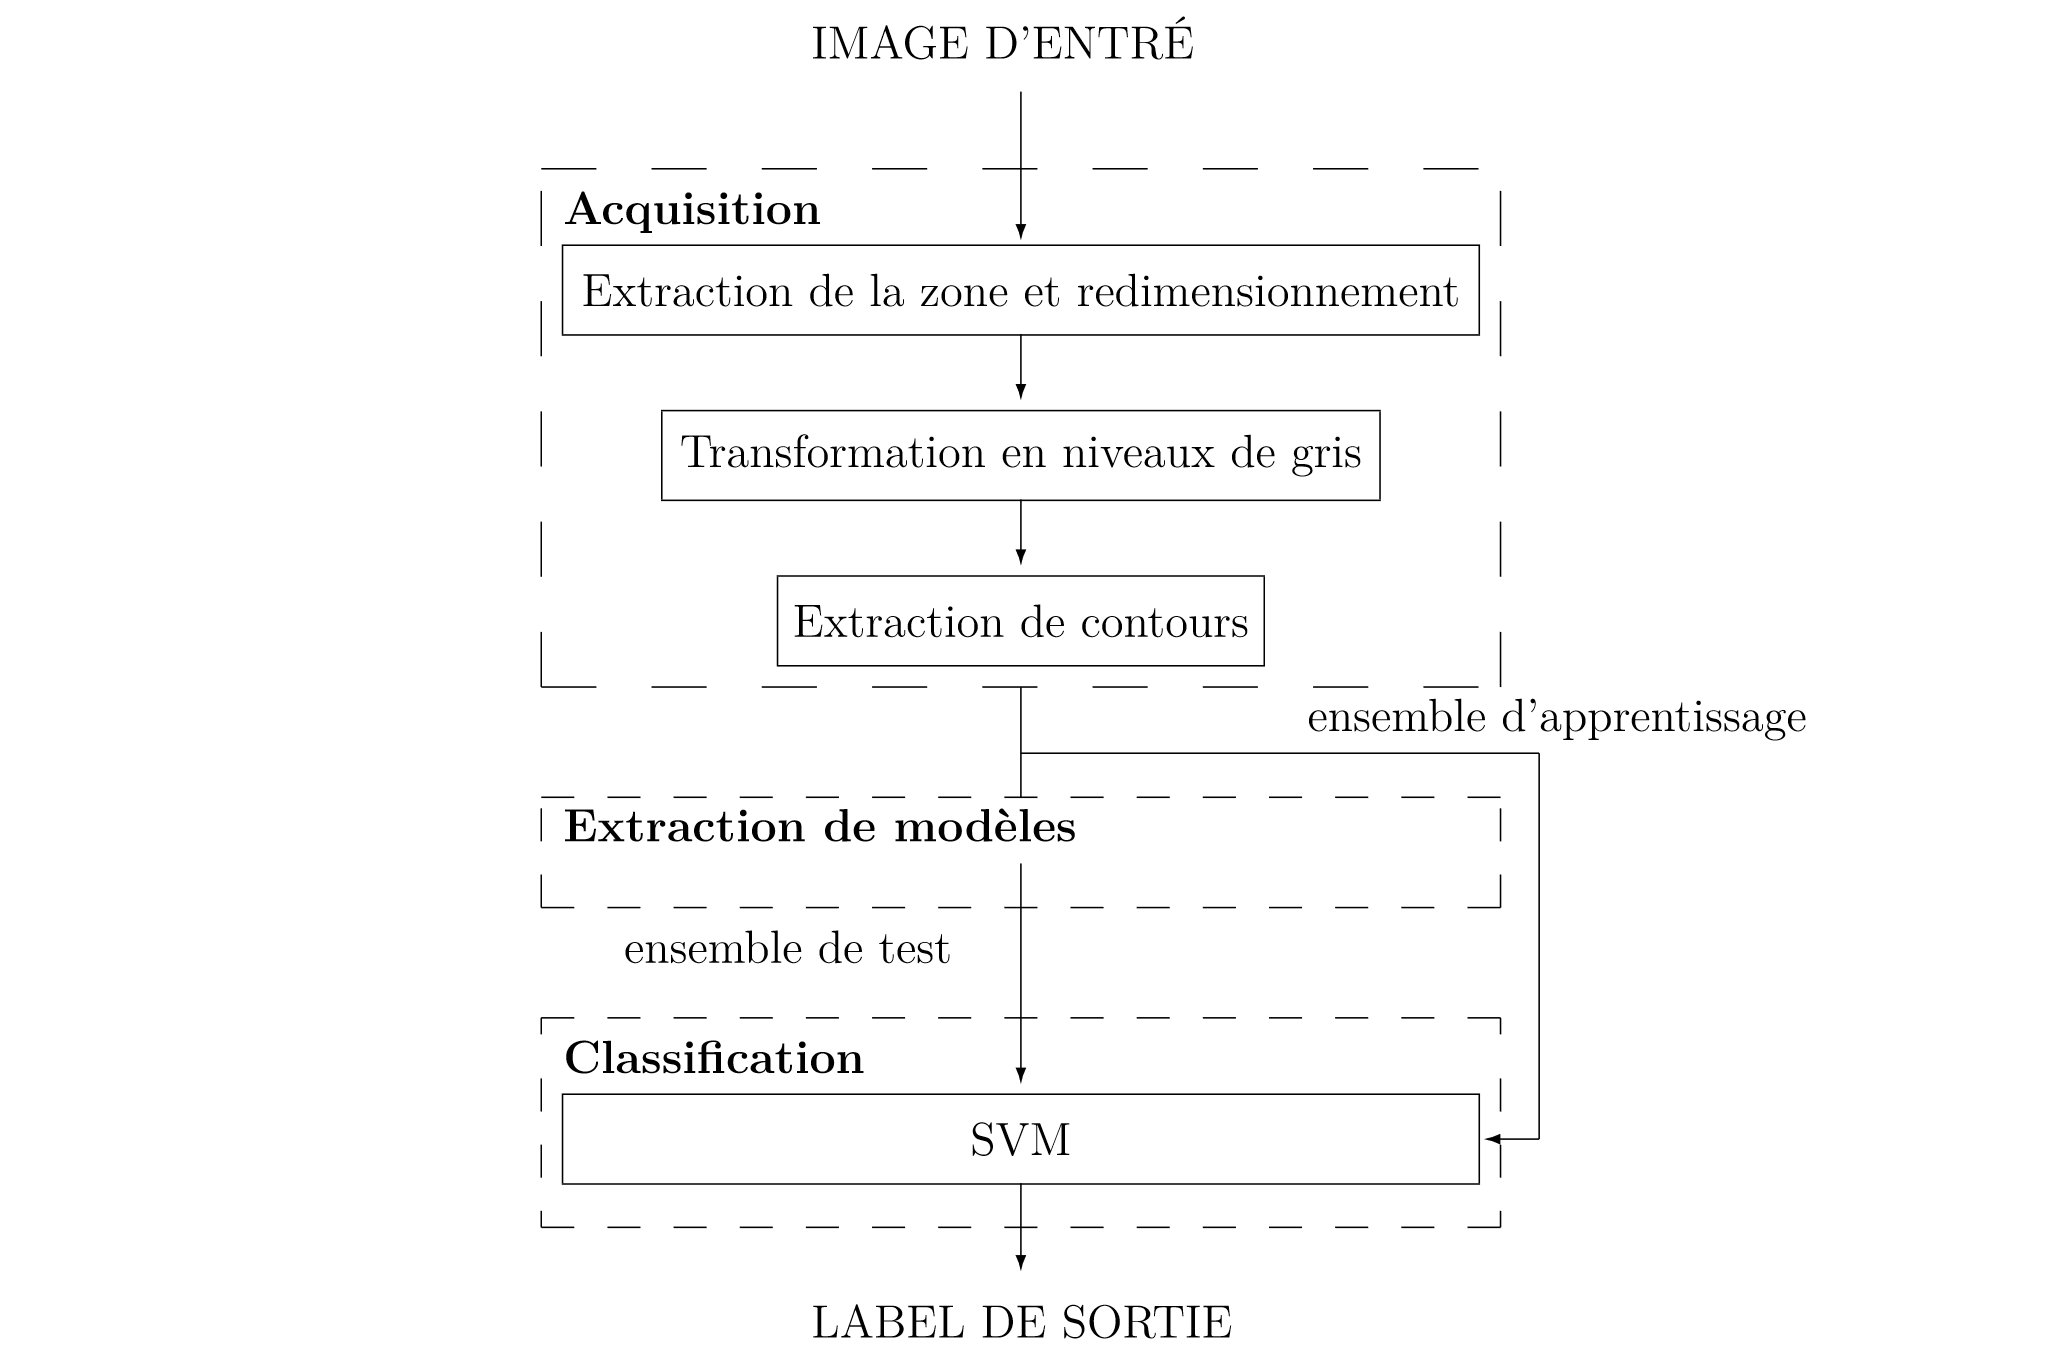
\includegraphics[scale=0.13]{image/test_exp.png}
        \end{figure}
    \end{columns}
\end{frame}

%------------------------------------------------

\subsection{Le protocole expérimental}
\begin{frame}
  \frametitle{Le protocole expérimental}
  \begin{figure}
    \centering
    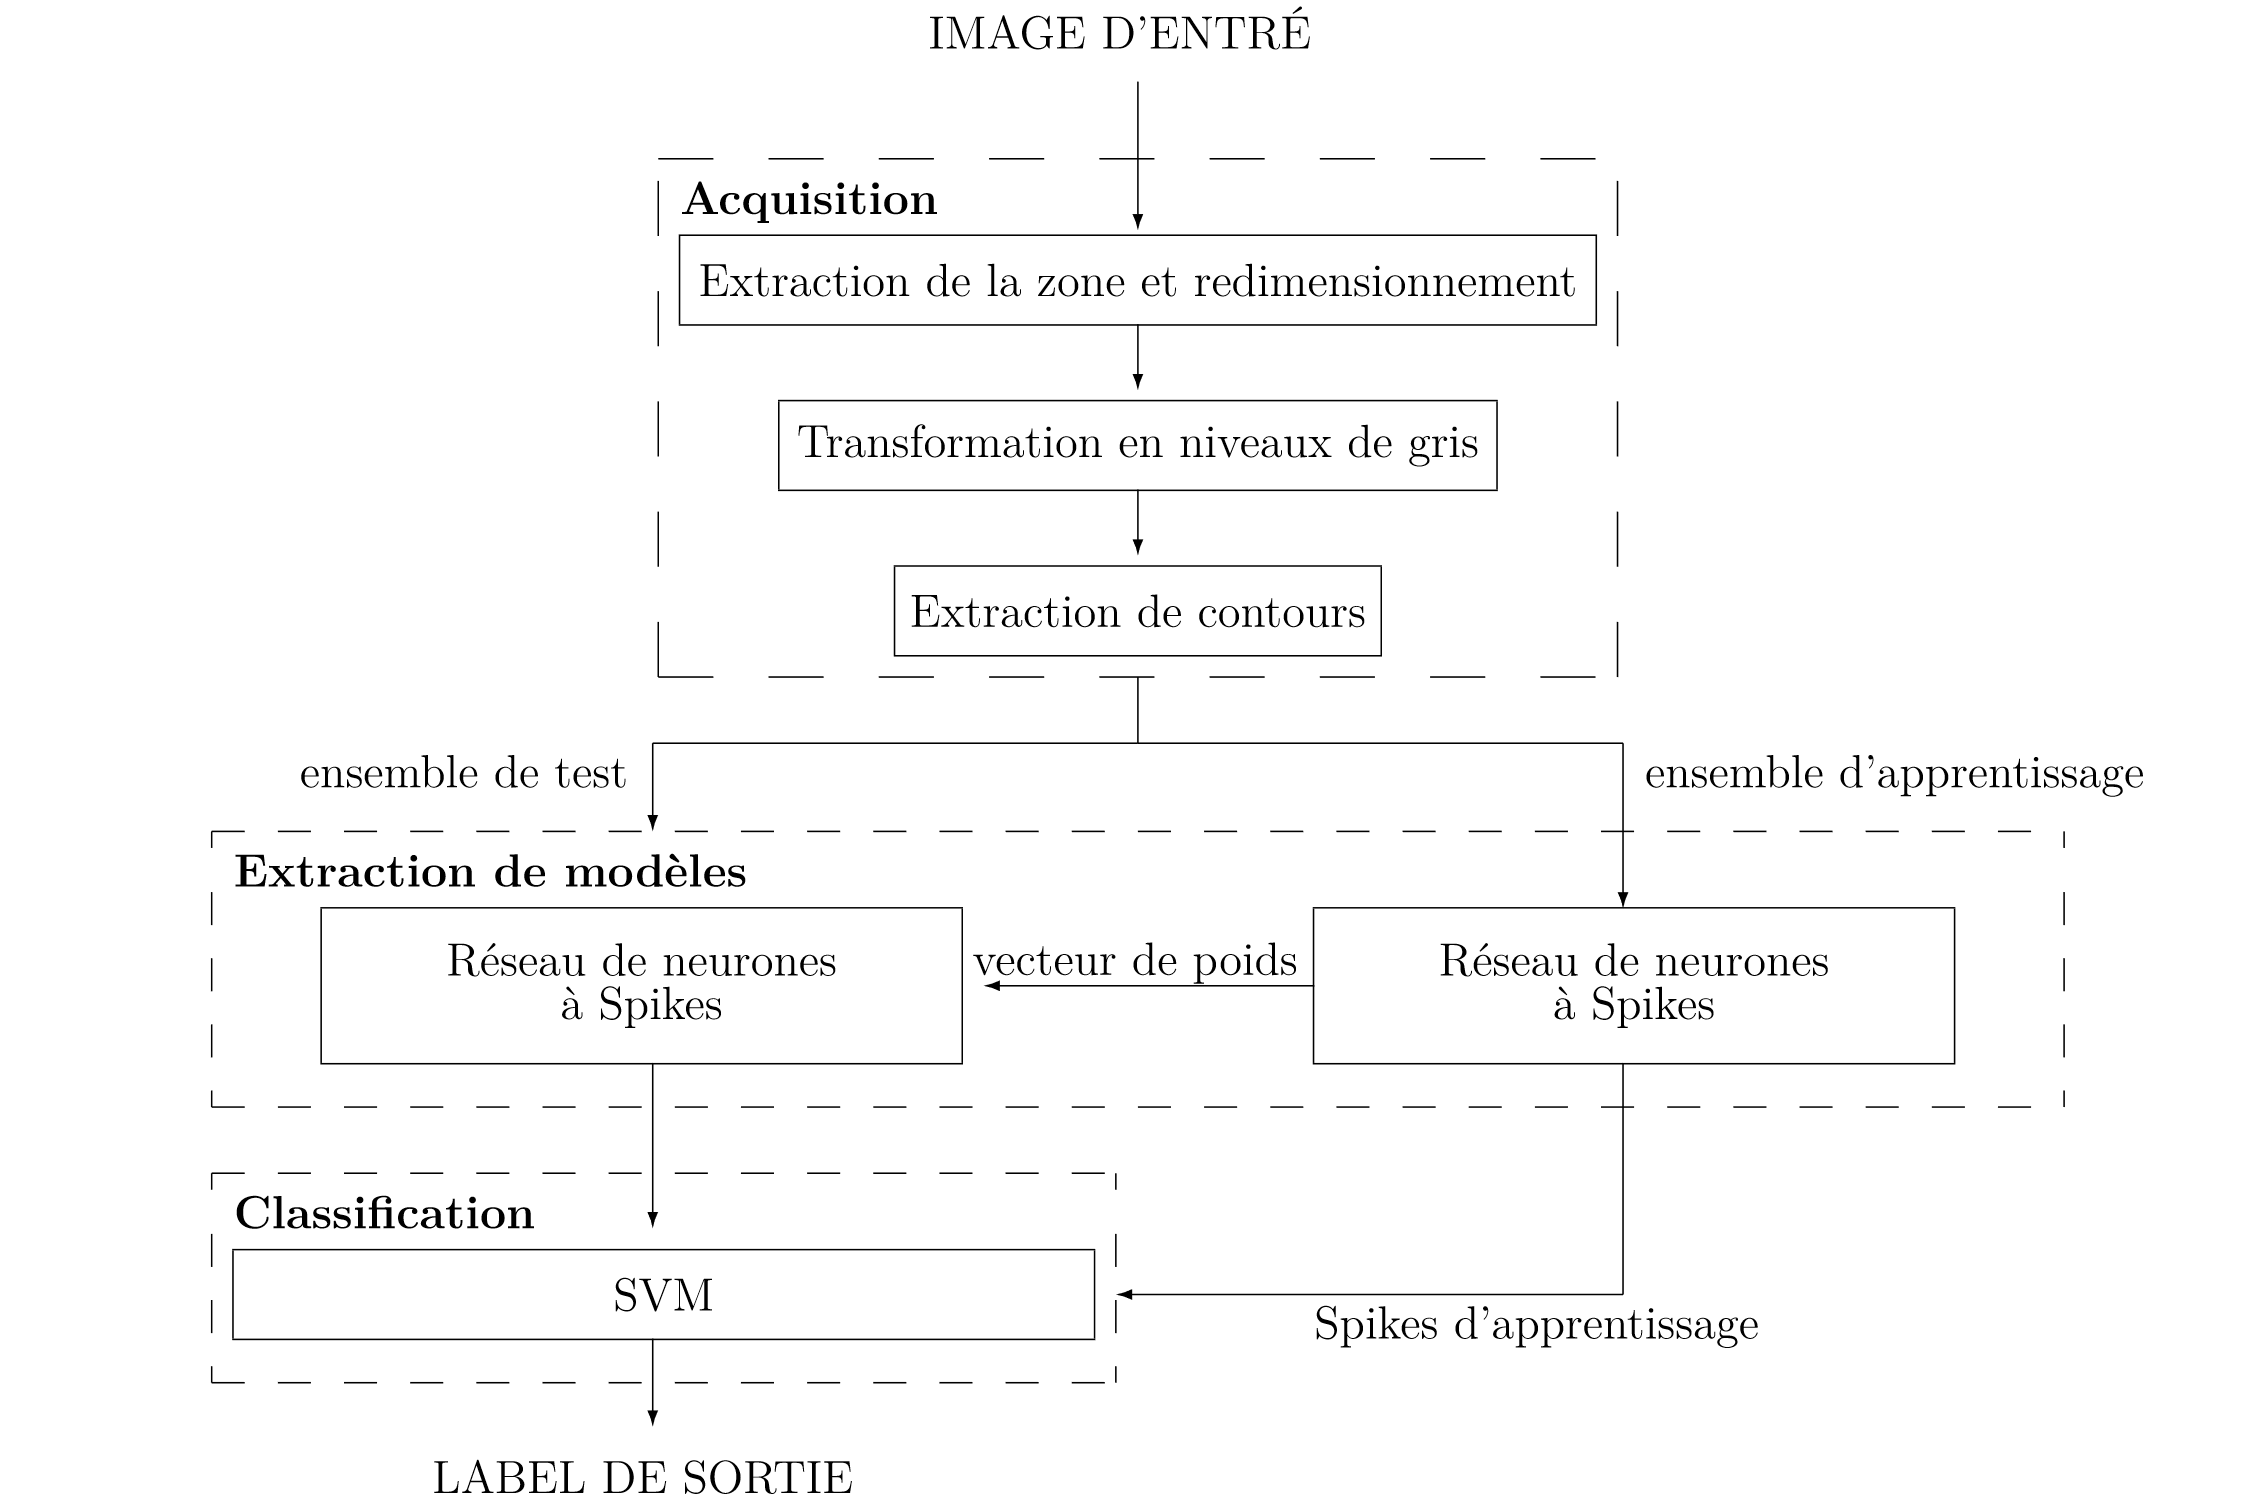
\includegraphics[scale=0.13]{image/archi.png}
  \end{figure}
\end{frame}

%------------------------------------------------

\end{document}